\section{Introduction} \label{sec:intro}

\section{Motivation}
Shortest Path (SP) calculation is much slower than retrieval from cache (\ffh{figure  out how by how much (possibly for more than one SP algorithm)})

Users want fast responsetime (and \spath can do this cheaper with caching \cite{ref.})

\spath service providers want to spend less money on hardware (less computation -> less hardware)

it is not feasable to store all possible \spaths (even if considering OSS)

Develop a caching scheme useable in domains wiht large set of opssible cacheable items and little or no  locality in new items added to system, or suggested added to cache.

No previous work has been done on cacheing \spath query results. interesting problem

More users now have a GPS and Web enabled mobile devices which makes \spath services more popular, but also require them to serve much larger set of users.








% 
% \subsubsection{OSC - Optimal Substructure Cache}
% OSC is more advanced than the two previous proposed solutions and therefor the scenario has been updated in figure . 
% To further improve upon Improved Baseline we will again utilize the optimal substructure, making it possible to have much fewer items in cache and still retain a high cache hit percentage \cite{ref}. %(assumption, need test result or proof), 
% Results with sub-paths shared by many users and longer, rather than short, paths are preferred to increase the utility of the cached shortest-path results.
% 
% By adding a more intuitive cache replacement policy which takes in to consideration both the usage of each cache item, as well as the coverage of previously often seen queries it is likely that the utility of the cache would be much higher. This addition is shown with the addition of the "`add to cache"' box in figure \ref{fig:advancedroutequery}B, added to show a heuristic\footnote{the actual heuristic will of cause only be defined later} will be used instead of a very simple method like LRU.


%\paragraph{\textbf{Number 3, ideas}}
%use optimal substructure\\
%prefer having longer paths in cache\\
%prefer having paths with subpaths shared by many users\\
%look at utility of cache items, not just usage when designing cache replacement policy.\\
%\begin{itemize}
%\item	prefer often used cache items
%\item	prefer items which cover routes/areas often used in previous queries
%\end{itemize}


\begin{figure}
  \center
	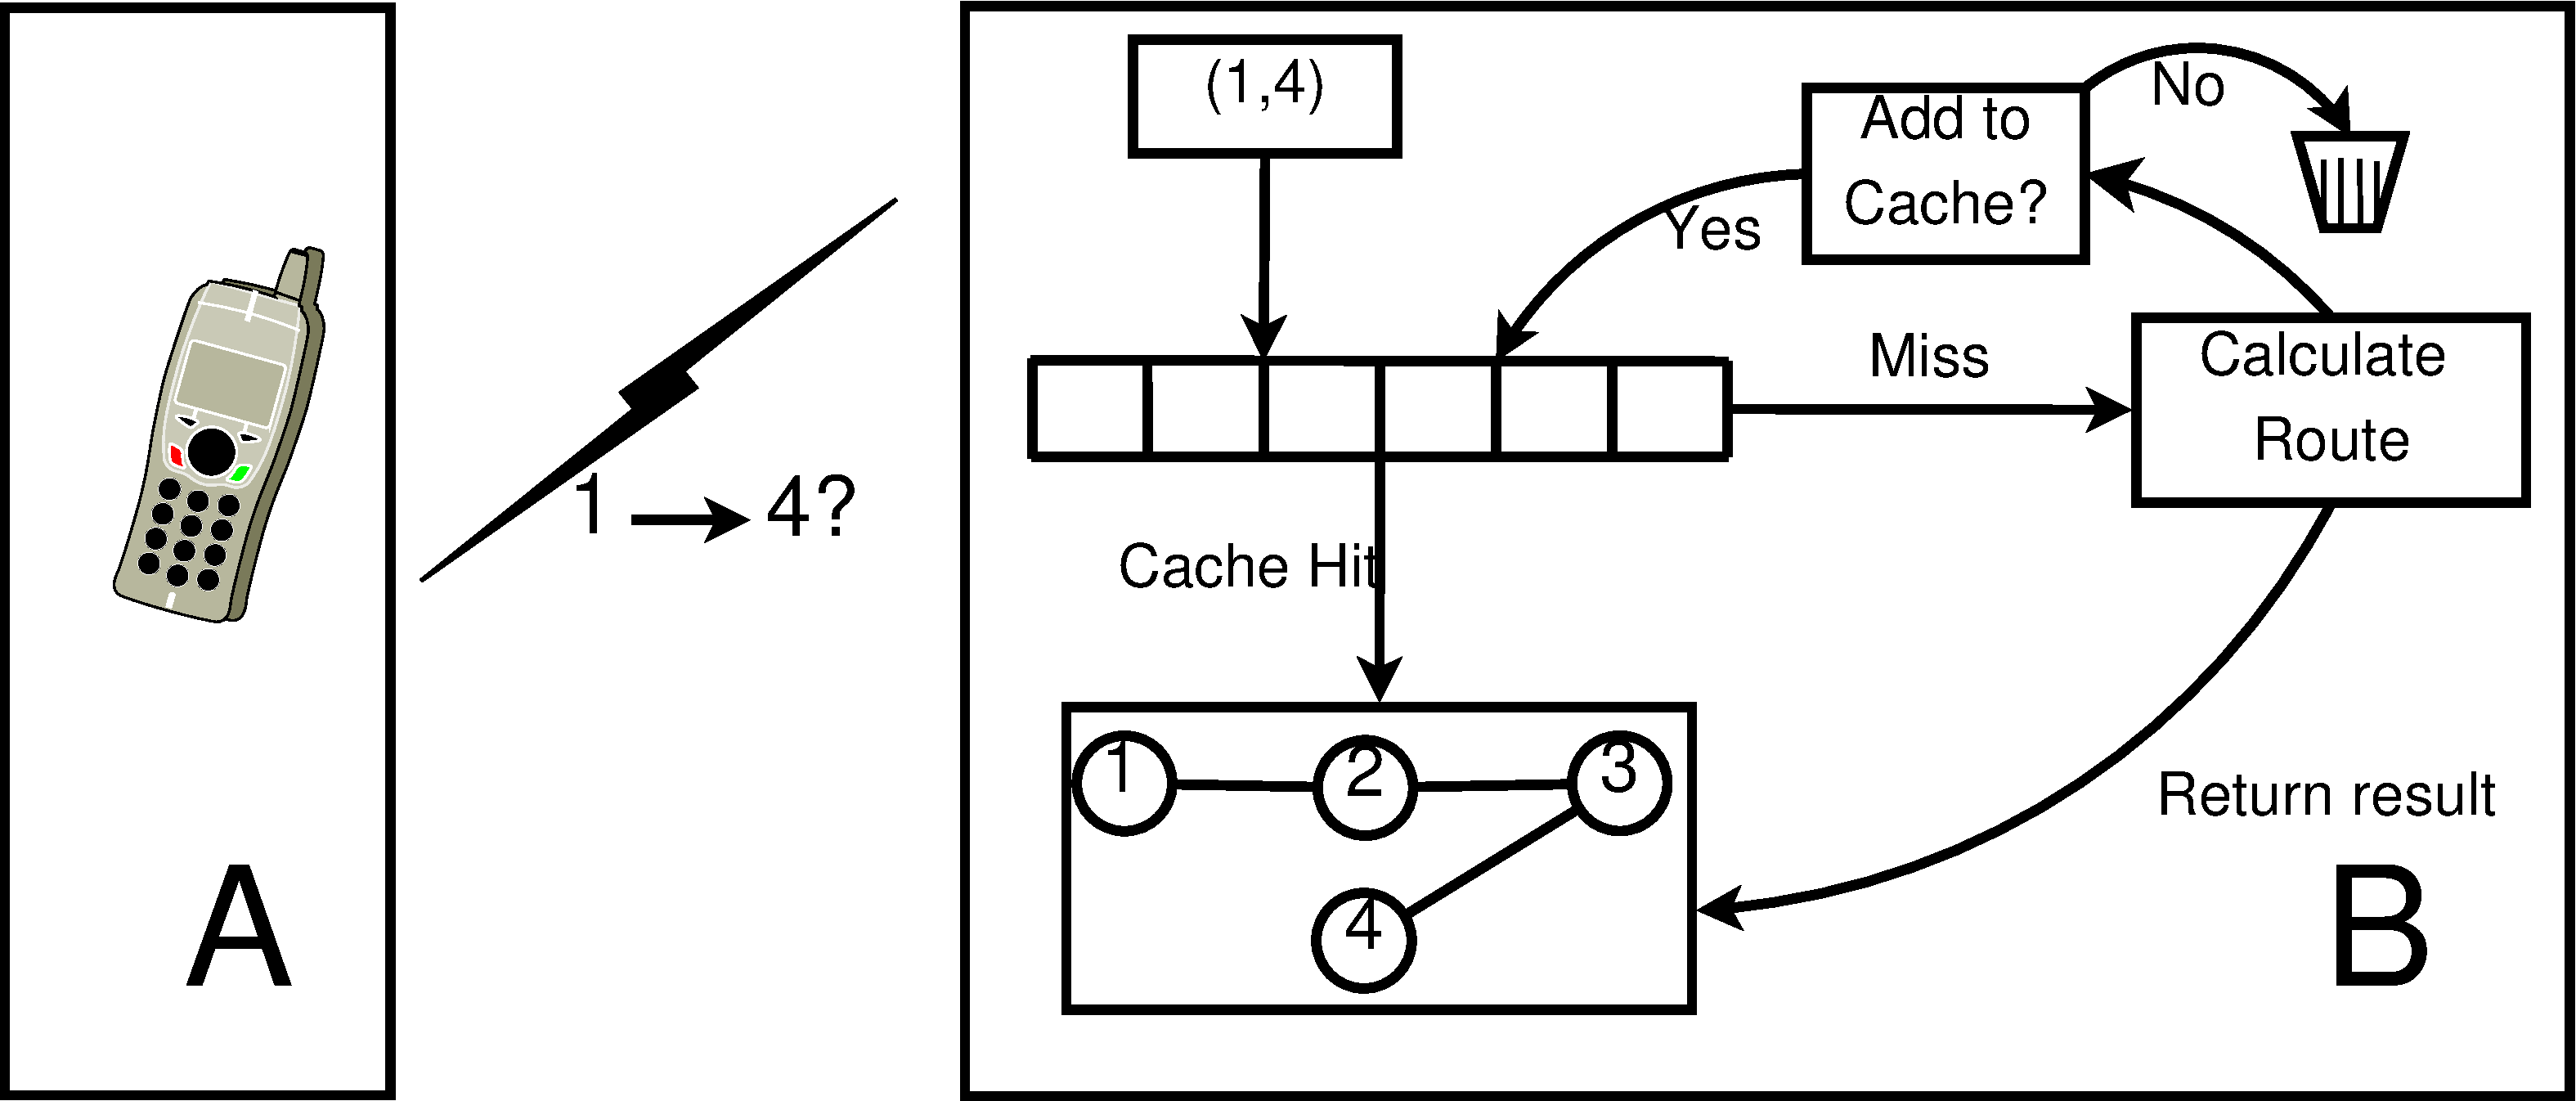
\includegraphics[width=0.5\textwidth]{figures/advancedroutequery.pdf}
	\caption{Advanced graph}
  \label{fig:advancedroutequery}
\end{figure}



%\paragraph{crap}
%We assume a setting where all users are equipped
%with a Mobile Device (MD) able to communicate and
%report the users position. All MDs are online and are
%continuesly reporting the users location at predetermined
%intervals. We use the terms user, mobile device, and
%client interchangeable and denote the set of MDs by
%UN. We expect a MD to be cabable of visualizing
%its current location.
%We assume a 2D scenario, where the movements of
%users uU are restricted to a road network G(V, E).
%V is the set of vertices, where each vertice v ∈ V
%represents either a street intersection or an important
%landmark. E is the set of directed edges augmented
%by edge length and type. Edges are represented by
%a begin/end vertice pair and each edge represents the
%smallest unit of a road segment. e ∈ E, each e being
%a tuple specifying id, start-/end-vertices, length, and
%Road Type (RT) (eid , vs , ve , elength , eRT ). RT is a
%hierarchy of the size/type of road i.e. highway, paved,
%or dirt road (Sec. 5.2).
%The simplest form of trajectory is a collection of tu-
%ples (time, longitude, latitude), ordered by the time
%attribute, but as we will work on a road network and
%in the spatio-temporal domain, such a basic notion of
%trajectories is not appropriate. We de�ne T as the set
%of trajectories, where each trajectory consist of an id
%(tid ), and a sequence of tuples containing an edge and



